% !TeX program = xelatex
\documentclass[12pt, a4paper]{article}
\usepackage{amsmath}
\usepackage{xeCJK}
\usepackage{amsmath}
\usepackage{amssymb}
\usepackage{xcolor}
\usepackage{parskip}
\usepackage{tikz}

\setmainfont{Latin Modern Roman}
\setCJKmainfont{Noto Serif CJK TC}

\title{BJT}

\begin{document}
\section*{Concept of BJT}
\begin{center}
	

\tikzset{every picture/.style={line width=0.75pt}} %set default line width to 0.75pt        

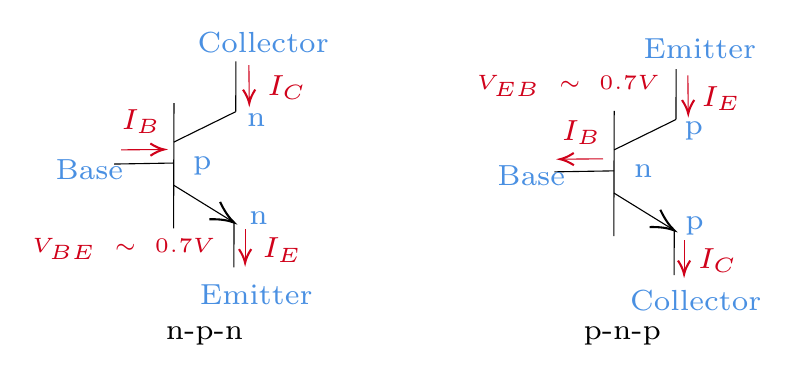
\begin{tikzpicture}[x=0.75pt,y=0.75pt,yscale=-1,xscale=1]
%uncomment if require: \path (0,300); %set diagram left start at 0, and has height of 300

%Straight Lines [id:da41720361884938184] 
\draw    (456.19,110.91) -- (456.13,129.72) -- (456.1,139.82) -- (456.07,150.51) -- (456,171.26) ;
%Straight Lines [id:da6884450440198249] 
\draw    (456.13,129.72) -- (485.95,115.07) ;
%Straight Lines [id:da4299314098075526] 
\draw    (456.07,150.51) -- (483.43,167.42) ;
\draw [shift={(485.13,168.47)}, rotate = 211.73] [color={rgb, 255:red, 0; green, 0; blue, 0 }  ][line width=0.75]    (10.93,-4.9) .. controls (6.95,-2.3) and (3.31,-0.67) .. (0,0) .. controls (3.31,0.67) and (6.95,2.3) .. (10.93,4.9)   ;
%Straight Lines [id:da99953250770795] 
\draw    (485.95,115.07) -- (486.03,90.84) ;
%Straight Lines [id:da16894446125496687] 
\draw    (485.13,168.47) -- (485.03,190.07) ;
%Straight Lines [id:da27628282565223083] 
\draw    (427.38,140.3) -- (456.1,139.82) ;
%Straight Lines [id:da5756441571661479] 
\draw    (244.09,107.15) -- (244.03,125.96) -- (244,136.05) -- (243.97,146.74) -- (243.9,167.49) ;
%Straight Lines [id:da06709557802156885] 
\draw    (244.03,125.96) -- (273.85,111.3) ;
%Straight Lines [id:da5280630440607302] 
\draw    (243.97,146.74) -- (271.33,163.66) ;
\draw [shift={(273.03,164.71)}, rotate = 211.73] [color={rgb, 255:red, 0; green, 0; blue, 0 }  ][line width=0.75]    (10.93,-4.9) .. controls (6.95,-2.3) and (3.31,-0.67) .. (0,0) .. controls (3.31,0.67) and (6.95,2.3) .. (10.93,4.9)   ;
%Straight Lines [id:da836552250786984] 
\draw    (273.85,111.3) -- (273.93,87.07) ;
%Straight Lines [id:da30921103922378723] 
\draw    (273.03,164.71) -- (272.93,186.3) ;
%Straight Lines [id:da18564800925517488] 
\draw    (215.28,136.54) -- (244,136.05) ;
%Straight Lines [id:da26678801997549273] 
\draw [color={rgb, 255:red, 208; green, 2; blue, 27 }  ,draw opacity=1 ]   (432.16,134.18) -- (450.79,134.02) ;
\draw [shift={(430.16,134.2)}, rotate = 359.51] [color={rgb, 255:red, 208; green, 2; blue, 27 }  ,draw opacity=1 ][line width=0.75]    (6.56,-2.94) .. controls (4.17,-1.38) and (1.99,-0.4) .. (0,0) .. controls (1.99,0.4) and (4.17,1.38) .. (6.56,2.94)   ;
%Straight Lines [id:da8448156798036344] 
\draw [color={rgb, 255:red, 208; green, 2; blue, 27 }  ,draw opacity=1 ]   (491.84,110.24) -- (491.68,93.87) ;
\draw [shift={(491.86,112.24)}, rotate = 269.46] [color={rgb, 255:red, 208; green, 2; blue, 27 }  ,draw opacity=1 ][line width=0.75]    (6.56,-2.94) .. controls (4.17,-1.38) and (1.99,-0.4) .. (0,0) .. controls (1.99,0.4) and (4.17,1.38) .. (6.56,2.94)   ;
%Straight Lines [id:da45090343003545064] 
\draw [color={rgb, 255:red, 208; green, 2; blue, 27 }  ,draw opacity=1 ]   (489.86,187.6) -- (489.86,173.31) ;
\draw [shift={(489.86,189.6)}, rotate = 270] [color={rgb, 255:red, 208; green, 2; blue, 27 }  ,draw opacity=1 ][line width=0.75]    (6.56,-2.94) .. controls (4.17,-1.38) and (1.99,-0.4) .. (0,0) .. controls (1.99,0.4) and (4.17,1.38) .. (6.56,2.94)   ;
%Straight Lines [id:da08583927969420024] 
\draw [color={rgb, 255:red, 208; green, 2; blue, 27 }  ,draw opacity=1 ]   (280.34,105.24) -- (280.18,88.87) ;
\draw [shift={(280.36,107.24)}, rotate = 269.46] [color={rgb, 255:red, 208; green, 2; blue, 27 }  ,draw opacity=1 ][line width=0.75]    (6.56,-2.94) .. controls (4.17,-1.38) and (1.99,-0.4) .. (0,0) .. controls (1.99,0.4) and (4.17,1.38) .. (6.56,2.94)   ;
%Straight Lines [id:da23637271134315985] 
\draw [color={rgb, 255:red, 208; green, 2; blue, 27 }  ,draw opacity=1 ]   (278.36,182.1) -- (278.36,167.81) ;
\draw [shift={(278.36,184.1)}, rotate = 270] [color={rgb, 255:red, 208; green, 2; blue, 27 }  ,draw opacity=1 ][line width=0.75]    (6.56,-2.94) .. controls (4.17,-1.38) and (1.99,-0.4) .. (0,0) .. controls (1.99,0.4) and (4.17,1.38) .. (6.56,2.94)   ;
%Straight Lines [id:da4645166143519025] 
\draw [color={rgb, 255:red, 208; green, 2; blue, 27 }  ,draw opacity=1 ]   (218.66,129.7) -- (237.29,129.54) ;
\draw [shift={(239.29,129.52)}, rotate = 179.51] [color={rgb, 255:red, 208; green, 2; blue, 27 }  ,draw opacity=1 ][line width=0.75]    (6.56,-2.94) .. controls (4.17,-1.38) and (1.99,-0.4) .. (0,0) .. controls (1.99,0.4) and (4.17,1.38) .. (6.56,2.94)   ;

% Text Node
\draw (253.62,71.1) node [anchor=north west][inner sep=0.75pt]  [font=\scriptsize,color={rgb, 255:red, 74; green, 144; blue, 226 }  ,opacity=1 ,xscale=1.5,yscale=1.5] [align=left] {Collector};
% Text Node
\draw (462.02,195.57) node [anchor=north west][inner sep=0.75pt]  [font=\scriptsize,color={rgb, 255:red, 74; green, 144; blue, 226 }  ,opacity=1 ,xscale=1.5,yscale=1.5] [align=left] {Collector};
% Text Node
\draw (254.72,192.8) node [anchor=north west][inner sep=0.75pt]  [font=\scriptsize,color={rgb, 255:red, 74; green, 144; blue, 226 }  ,opacity=1 ,xscale=1.5,yscale=1.5] [align=left] {Emitter};
% Text Node
\draw (468.42,74.14) node [anchor=north west][inner sep=0.75pt]  [font=\scriptsize,color={rgb, 255:red, 74; green, 144; blue, 226 }  ,opacity=1 ,xscale=1.5,yscale=1.5] [align=left] {Emitter};
% Text Node
\draw (398.02,135.17) node [anchor=north west][inner sep=0.75pt]  [font=\scriptsize,color={rgb, 255:red, 74; green, 144; blue, 226 }  ,opacity=1 ,xscale=1.5,yscale=1.5] [align=left] {Base};
% Text Node
\draw (185.12,132.37) node [anchor=north west][inner sep=0.75pt]  [font=\scriptsize,color={rgb, 255:red, 74; green, 144; blue, 226 }  ,opacity=1 ,xscale=1.5,yscale=1.5] [align=left] {Base};
% Text Node
\draw (463.91,135.17) node [anchor=north west][inner sep=0.75pt]  [font=\scriptsize,color={rgb, 255:red, 74; green, 144; blue, 226 }  ,opacity=1 ,xscale=1.5,yscale=1.5] [align=left] {n};
% Text Node
\draw (277.41,110.33) node [anchor=north west][inner sep=0.75pt]  [font=\scriptsize,color={rgb, 255:red, 74; green, 144; blue, 226 }  ,opacity=1 ,xscale=1.5,yscale=1.5] [align=left] {n};
% Text Node
\draw (278.57,157.83) node [anchor=north west][inner sep=0.75pt]  [font=\scriptsize,color={rgb, 255:red, 74; green, 144; blue, 226 }  ,opacity=1 ,xscale=1.5,yscale=1.5] [align=left] {n};
% Text Node
\draw (488.19,114.4) node [anchor=north west][inner sep=0.75pt]  [font=\scriptsize,color={rgb, 255:red, 74; green, 144; blue, 226 }  ,opacity=1 ,xscale=1.5,yscale=1.5] [align=left] {p};
% Text Node
\draw (488.57,160.12) node [anchor=north west][inner sep=0.75pt]  [font=\scriptsize,color={rgb, 255:red, 74; green, 144; blue, 226 }  ,opacity=1 ,xscale=1.5,yscale=1.5] [align=left] {p};
% Text Node
\draw (251.41,131) node [anchor=north west][inner sep=0.75pt]  [font=\scriptsize,color={rgb, 255:red, 74; green, 144; blue, 226 }  ,opacity=1 ,xscale=1.5,yscale=1.5] [align=left] {p};
% Text Node
\draw (439.57,213.33) node [anchor=north west][inner sep=0.75pt]  [font=\scriptsize,xscale=1.5,yscale=1.5] [align=left] {p-n-p};
% Text Node
\draw (238.24,213.17) node [anchor=north west][inner sep=0.75pt]  [font=\scriptsize,xscale=1.5,yscale=1.5] [align=left] {n-p-n};
% Text Node
\draw (429.21,113.85) node [anchor=north west][inner sep=0.75pt]  [font=\scriptsize,color={rgb, 255:red, 208; green, 2; blue, 27 }  ,opacity=1 ,xscale=1.5,yscale=1.5]  {$I_{B}$};
% Text Node
\draw (496.54,97.27) node [anchor=north west][inner sep=0.75pt]  [font=\scriptsize,color={rgb, 255:red, 208; green, 2; blue, 27 }  ,opacity=1 ,xscale=1.5,yscale=1.5]  {$I_{E}$};
% Text Node
\draw (494.83,175.51) node [anchor=north west][inner sep=0.75pt]  [font=\scriptsize,color={rgb, 255:red, 208; green, 2; blue, 27 }  ,opacity=1 ,xscale=1.5,yscale=1.5]  {$I_{C}$};
% Text Node
\draw (388.03,91.81) node [anchor=north west][inner sep=0.75pt]  [font=\tiny,color={rgb, 255:red, 208; green, 2; blue, 27 }  ,opacity=1 ,xscale=1.5,yscale=1.5]  {$V_{EB} \ \sim \ 0.7V$};
% Text Node
\draw (285.04,170.27) node [anchor=north west][inner sep=0.75pt]  [font=\scriptsize,color={rgb, 255:red, 208; green, 2; blue, 27 }  ,opacity=1 ,xscale=1.5,yscale=1.5]  {$I_{E}$};
% Text Node
\draw (287.33,92.01) node [anchor=north west][inner sep=0.75pt]  [font=\scriptsize,color={rgb, 255:red, 208; green, 2; blue, 27 }  ,opacity=1 ,xscale=1.5,yscale=1.5]  {$I_{C}$};
% Text Node
\draw (217.04,108.35) node [anchor=north west][inner sep=0.75pt]  [font=\scriptsize,color={rgb, 255:red, 208; green, 2; blue, 27 }  ,opacity=1 ,xscale=1.5,yscale=1.5]  {$I_{B}$};
% Text Node
\draw (173.87,170.31) node [anchor=north west][inner sep=0.75pt]  [font=\tiny,color={rgb, 255:red, 208; green, 2; blue, 27 }  ,opacity=1 ,xscale=1.5,yscale=1.5]  {$V_{BE} \ \sim \ 0.7V$};
\end{tikzpicture}
\end{center}

\subsection*{Active mode}
B-E junction: \textbf{Forward bias} $\sim 0.7$V in general \\
B-C junction: \textbf{Reverse bias} or forward bias $<0.4$V

\subsection*{Saturation mode}
B-E junction: forward bias\\
B-C junction: forward bias \textcolor{red}> \textcolor{black}0.4V

\subsection*{Reverse active(Cut-off)}
B-E junction: reverse bias\\
B-C junction: forward bias
\newpage

\section*{Equation of BJT}

\begin{center}
\tikzset{every picture/.style={line width=0.75pt}} %set default line width to 0.75pt        

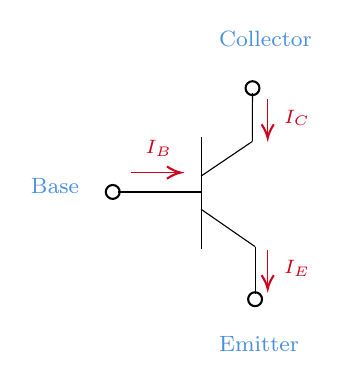
\begin{tikzpicture}[x=0.75pt,y=0.75pt,yscale=-1,xscale=1]
%uncomment if require: \path (0,300); %set diagram left start at 0, and has height of 300

%Straight Lines [id:da21757148579979202] 
\draw    (270.52,94.89) -- (270.52,113.56) -- (270.52,121.21) -- (270.52,129.56) -- (270.52,148.89) ;
%Straight Lines [id:da25534728237338333] 
\draw    (270.52,113.56) -- (295.18,96.89) ;
%Straight Lines [id:da07586494603654681] 
\draw    (270.52,129.56) -- (296.52,147.56) ;
%Straight Lines [id:da7075217700722117] 
\draw    (296.52,147.56) -- (296.52,170.54) ;
\draw [shift={(296.52,172.89)}, rotate = 90] [color={rgb, 255:red, 0; green, 0; blue, 0 }  ][line width=0.75]      (0, 0) circle [x radius= 3.35, y radius= 3.35]   ;
%Straight Lines [id:da7681202035592422] 
\draw    (295.26,73.56) -- (295.18,96.89) ;
\draw [shift={(295.27,71.21)}, rotate = 90.19] [color={rgb, 255:red, 0; green, 0; blue, 0 }  ][line width=0.75]      (0, 0) circle [x radius= 3.35, y radius= 3.35]   ;
%Straight Lines [id:da06169247997439231] 
\draw    (230.29,121.21) -- (270.52,121.21) ;
\draw [shift={(227.94,121.21)}, rotate = 0] [color={rgb, 255:red, 0; green, 0; blue, 0 }  ][line width=0.75]      (0, 0) circle [x radius= 3.35, y radius= 3.35]   ;
%Straight Lines [id:da6741645038870837] 
\draw [color={rgb, 255:red, 208; green, 2; blue, 27 }  ,draw opacity=1 ]   (236.6,111.88) -- (258.6,111.88) ;
\draw [shift={(260.6,111.88)}, rotate = 180] [color={rgb, 255:red, 208; green, 2; blue, 27 }  ,draw opacity=1 ][line width=0.75]    (6.56,-2.94) .. controls (4.17,-1.38) and (1.99,-0.4) .. (0,0) .. controls (1.99,0.4) and (4.17,1.38) .. (6.56,2.94)   ;
%Straight Lines [id:da794298671098817] 
\draw [color={rgb, 255:red, 208; green, 2; blue, 27 }  ,draw opacity=1 ]   (302.6,76.54) -- (302.6,93.21) ;
\draw [shift={(302.6,95.21)}, rotate = 270] [color={rgb, 255:red, 208; green, 2; blue, 27 }  ,draw opacity=1 ][line width=0.75]    (6.56,-2.94) .. controls (4.17,-1.38) and (1.99,-0.4) .. (0,0) .. controls (1.99,0.4) and (4.17,1.38) .. (6.56,2.94)   ;
%Straight Lines [id:da8468813132864502] 
\draw [color={rgb, 255:red, 208; green, 2; blue, 27 }  ,draw opacity=1 ]   (302.6,149.21) -- (302.6,165.88) ;
\draw [shift={(302.6,167.88)}, rotate = 270] [color={rgb, 255:red, 208; green, 2; blue, 27 }  ,draw opacity=1 ][line width=0.75]    (6.56,-2.94) .. controls (4.17,-1.38) and (1.99,-0.4) .. (0,0) .. controls (1.99,0.4) and (4.17,1.38) .. (6.56,2.94)   ;

% Text Node
\draw (242.55,95.07) node [anchor=north west][inner sep=0.75pt]  [font=\scriptsize,color={rgb, 255:red, 208; green, 2; blue, 27 }  ,opacity=1 ]  {$I_{B}$};
% Text Node
\draw (309.22,80.4) node [anchor=north west][inner sep=0.75pt]  [font=\scriptsize,color={rgb, 255:red, 208; green, 2; blue, 27 }  ,opacity=1 ]  {$I_{C}$};
% Text Node
\draw (309.22,153.07) node [anchor=north west][inner sep=0.75pt]  [font=\scriptsize,color={rgb, 255:red, 208; green, 2; blue, 27 }  ,opacity=1 ]  {$I_{E}$};
% Text Node
\draw (277.88,42.33) node [anchor=north west][inner sep=0.75pt]  [font=\footnotesize,color={rgb, 255:red, 74; green, 144; blue, 226 }  ,opacity=1 ] [align=left] {Collector};
% Text Node
\draw (277.88,189.67) node [anchor=north west][inner sep=0.75pt]  [font=\footnotesize,color={rgb, 255:red, 74; green, 144; blue, 226 }  ,opacity=1 ] [align=left] {Emitter};
% Text Node
\draw (187.22,113.33) node [anchor=north west][inner sep=0.75pt]  [font=\footnotesize,color={rgb, 255:red, 74; green, 144; blue, 226 }  ,opacity=1 ] [align=left] {Base};
\end{tikzpicture}
\end{center}

$i_C$ 有三種表示法
\begin{align*}
	i_C &= I_s \exp(\frac{V_{BE}}{V_T}) \\
	i_C &= \alpha i_E \\
	i_C &= \beta i_B
\end{align*}
By KCL, we have
\begin{align*}
	i_E &= i_C + i_B = (1 + \beta) i_B \\
	\alpha &= \frac{\beta}{1 + \beta}
\end{align*}

\subsection*{Activate Mode}
在Activate region 可以直接用$V_{BE} \sim 0.7$V 進行解題。 \\
算完後要確認 $V_{CE} > 0.3$V,如果沒有則為 Saturatino mode,要用 Saturation 再解一次 

\subsection*{Saturation Mode}
可以直接將 $V_{CE}$ 假設成 0.2V \\
$V_{BE}$ 一樣是用 0.7V 計算

\newpage


\section*{Early effect}



\end{document}
